\documentclass{beamer}

\usetheme{Warsaw}
\usefonttheme{professionalfonts}
%\logo{\includegraphics[height=1cm]{./images/logo.png}}
\beamertemplatenavigationsymbolsempty
\setbeamertemplate{caption}{\raggedright\insertcaption\par}
\usepackage{amsmath}
\usepackage{amssymb}
\usepackage[spanish]{babel}
\usepackage{changepage}
\usepackage{fancyvrb}
\usepackage{float}
\usepackage{framed}
\usepackage[T1]{fontenc}
\usepackage{geometry}
\usepackage{graphicx}
\usepackage{hyperref}
\usepackage[utf8]{inputenc}
\usepackage{minted}
\usepackage{multicol}
\usepackage{relsize}
\usepackage{subcaption}
\usepackage{textcomp}
\usepackage{tikz}
\usepackage{upgreek}
\usepackage{verbatim}
\usepackage{wasysym}
\usepackage{xcolor}
\definecolor{LightGray}{gray}{0.9}

%\setbeamertemplate{footline}[frame number]

\begin{document}

\title[Lógica proposicional]{Teoría de la Computación \\ Unidad 1: Lógica
  proposicional (parte 2)} \author[Teoría de la
Computación]{cristobal.loyola@usach.cl} \date{}

\titlegraphic{
  \vspace{-1.5cm}
  \begin{figure}
    \centering
    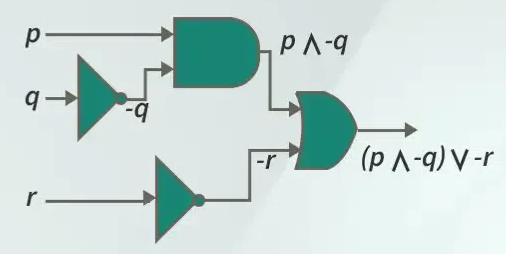
\includegraphics[width=.75\linewidth]{images/circuito_logico.png}
    \caption*{Diapositivas basadas en el material del profesor Daniel Vega}
  \end{figure}
}

\frame{\titlepage}

\setbeamertemplate{footline}[frame number]

\begin{frame}{Contenidos}
  Lógica proposicional: sintaxis
  \begin{itemize}
    \item Fórmula bien formada (FBF).
    \item Inducción estructural.
  \end{itemize}
\end{frame}


\begin{frame}{Lógica proposicional: Sintaxis}
  Definiremos un conjunto de símbolos (alfabeto) dado por:
  \begin{itemize}[<+->]
    \item Un conjunto P (posiblemente infinito) de variables proposicionales: $p$, $q$, $r$, $s$,...
    \item Constantes: V o F (1 o 0, T o F)
    \item Conectores lógicos: $\sim$, $\land$, $\vee$, $\rightarrow$,
          $\leftrightarrow$
    \item Símbolos de puntuación: (, )
  \end{itemize}
\end{frame}


\begin{frame}{Lógica proposicional: Sintaxis}
  A partir de un conjunto fijo P de variables, es posible definir un lenguaje
  proposicional L(P), que contiene todas las fórmulas posibles a través de una
  definición inductiva.\\

  Así, L(P) está formado por fórmulas, donde una fórmula es:
  \begin{itemize}
    \item Una constante o un elemento de P (fórmulas atómicas).
    \item Si $\upvarphi$ es una fórmula, entonces $\sim \upvarphi$ también es
          una fórmula.
    \item Si $\upvarphi$ y $\Uppsi$ son fórmulas, entonces
          ($\upvarphi \star \Uppsi$) es una fórmula ($\star$ representa
          cualquier conector binario).
  \end{itemize}

  \textbf{Definición:} en lógica proposicional, una fórmula bien formada (FBF)
  es aquella que es obtenida usando únicamente las reglas de construcción antes
  definidas una cantidad finita de veces.
\end{frame}


\begin{frame}{Lógica proposicional: Sintaxis}
  Definiciones inductivas, como la anterior, son muy frecuentes, tanto que se
  suelen definir empleando una gramática en Backus Naur Form (BNF). En esa
  forma, la definición anterior se lee de manera más compacta como:

  $$\upvarphi ::= p \,|\, (\sim \upvarphi) \,|\, (\upvarphi \land \upvarphi) \,|\,  (\upvarphi \vee \upvarphi) \,|\,  (\upvarphi \rightarrow \upvarphi) \,|\,  (\upvarphi \leftrightarrow \upvarphi)$$

  donde $p$ representa cualquier proposición atómica y cualquier ocurrencia de
  $\upvarphi$ a la derecha de ::= representa cualquier fórmula antes construida.
\end{frame}


\begin{frame}{Lógica proposicional: Sintaxis}
  ¿Son las siguientes expresiones FBF?
  \begin{itemize}
    \item $(p \vee q) \land q$
    \item $(p \land \sim q \sim) \land \vee r)$
  \end{itemize}
\end{frame}


\begin{frame}{Lógica proposicional: Sintaxis}
  \begin{itemize}[<+->]
    \item Sumemos los primeros 10 números naturales.
    \item Ahora, los 100 primeros naturales.
    \item ¿Y si queremos la suma de los 1000 primeros naturales?
    \item Se puede demostrar mediante inducción que:
    $$1 + 2 + 3 + ... + n = \dfrac{n (n+1)}{2}$$
  \end{itemize}
\end{frame}


\begin{frame}{Lógica proposicional: Sintaxis}
  La inducción matemática nos permite probar que determinada propiedad es
  satisfecha por cualquier número natural. Por ejemplo, para el caso anterior,
  basta definir $M(k)$ para indicar que la propiedad es satisfecha por $k$. Así,
  supongamos que conocemos las siguientes propiedades para $M$:\\

  \begin{itemize}
    \item \textbf{Caso base:} el número natural 1 satisface $M(1)$.
    \item \textbf{Paso inductivo:} se asume que la propiedad $M(n)$ es cierta
          para un determinado número natural $n$, luego se debe probar que para
          $n+1$ se satisface $M(n+1)$, es decir, existe una prueba de que $M(n) \rightarrow M(n+1)$.
  \end{itemize}
\end{frame}


\begin{frame}{Lógica proposicional: Sintaxis}
  \textbf{Definición:} sea $\upvarphi$ una FBF, definimos su altura como la suma
  entre 1 y el tamaño del camino más largo de su árbol de análisis sintáctico.\\

  Ya que cualquier FBF tiene tamaño finito, podemos mostrar declaraciones sobre
  todas las FBF por inducción matemática en sus alturas. Esta propiedad se
  conoce habitualmente como \textbf{inducción estructural}, técnica de
  razonamiento muy importante en ciencias de la computación. Por ejemplo:\\

  \textbf{Teorema:} para cada FBF, el número de paréntesis izquierdos es igual al número de paréntesis derechos.
\end{frame}


\begin{frame}{Lógica proposicional: Sintaxis}
  \textbf{Teorema:} para cada FBF, el número de paréntesis izquierdos es igual al número de paréntesis derechos.\\

  \textbf{Demostración:} usamos inducción sobre la altura de la FBF $\upvarphi$,
  definiendo $M(n)$ como “todas las fórmulas de altura $n$ tienen el mismo
  número de paréntesis izquierdos y derechos”. Luego, asumimos $M(k)$ para cada
  $k < n$ e intentamos probar $M(n)$.
\end{frame}


\begin{frame}{Lógica proposicional: Sintaxis}
  \textbf{Teorema:} para cada FBF, el número de paréntesis izquierdos es igual al número de paréntesis derechos.\\

  \textbf{Caso base (n=1):} en este caso $\upvarphi$ es una proposición atómica,
  por lo que no hay paréntesis izquierdos ni derechos, es decir, $0 = 0$.\\

  \textbf{Paso inductivo:} en este caso, el inicio del árbol sintáctico de
  $\upvarphi$ debe ser alguno de los conectores $\sim$, $\land$, $\vee$,
  $\rightarrow$ para que $\upvarphi$ sea una FBF. En particular y sin pérdida de
  generalidad, asumimos que es $\rightarrow$ (los otros casos siguen el mismo
  razonamiento). Luego, $\upvarphi$ equivale a
  $(\upvarphi_{1} \rightarrow \upvarphi_{2})$ para $\upvarphi_{1}$,
  $\upvarphi_{2}$ FBF ($\upvarphi_{1}$, $\upvarphi_{2}$ son las representaciones
  lineales de los subárboles izquierdo y derecho de $\upvarphi$). Dado que las
  alturas de $\upvarphi_{1}$ y $\upvarphi_{2}$ son estrictamente menores que
  $n$, usando la hipótesis inductiva, podemos concluir que $\upvarphi_{1}$ tiene
  el mismo número de paréntesis izquierdos y derechos, y lo mismo para
  $\upvarphi_{2}$. Pero en ($\upvarphi_{1} \rightarrow \upvarphi_{2}$) agregamos
  dos paréntesis más. Así, el número de ocurrencias de paréntesis izquierdos y
  derechos es el mismo.
\end{frame}


\end{document}
